\section{Quantification (Experiments): Planting a Shortcut Dials Headroom Down}
\label{sec:dose}

\paragraph{Design.}
In PMC-VQA, where the correct option is not the shortest, we plant the length shortcut at $d\in\{0.25,0.40,0.55,0.70,0.85,0.92\}$ and fine-tune Qwen2.5-VL-3B for each dose and three seeds (18 runs); we evaluate on the 1{,}999 clean test questions with the true image, a black image and the six-level visual ladder.
We define the \emph{visual veto boundary} $V^\ast$ as the weakest ladder level at which the image benefit $g$ reaches $+2$ points with a paired-bootstrap lower bound of at least $+1$; $V^\ast=\text{none}$ if no level qualifies (criterion fixed before the runs).

\paragraph{Three quantities, not to be confused.} The visual veto boundary $V^\ast$ and the \emph{lock-out} (the weakest tested shortcut strength at which $V^\ast$ is \emph{none}) were fixed before the PMC-VQA dose study (amendment A17), and the PMC-VQA lock-out of $0.85$ comes from that pre-specified grid. The A-OKVQA lock-out at $0.99$ is different: the criterion was fixed before the runs, but the strength was added after the $0.92$ prediction failed (A21, A22; Supp.~W). The $20\%$ relative criterion, the strength at which the benefit falls to a fifth of its value at $d=0.25$, is exploratory (Supp.~Y): it gives lower strengths ($0.74$ for Qwen-3B on PMC-VQA; $0.94$ on A-OKVQA) and is not a lock-out.

\begin{figure*}[t]
  \centering
  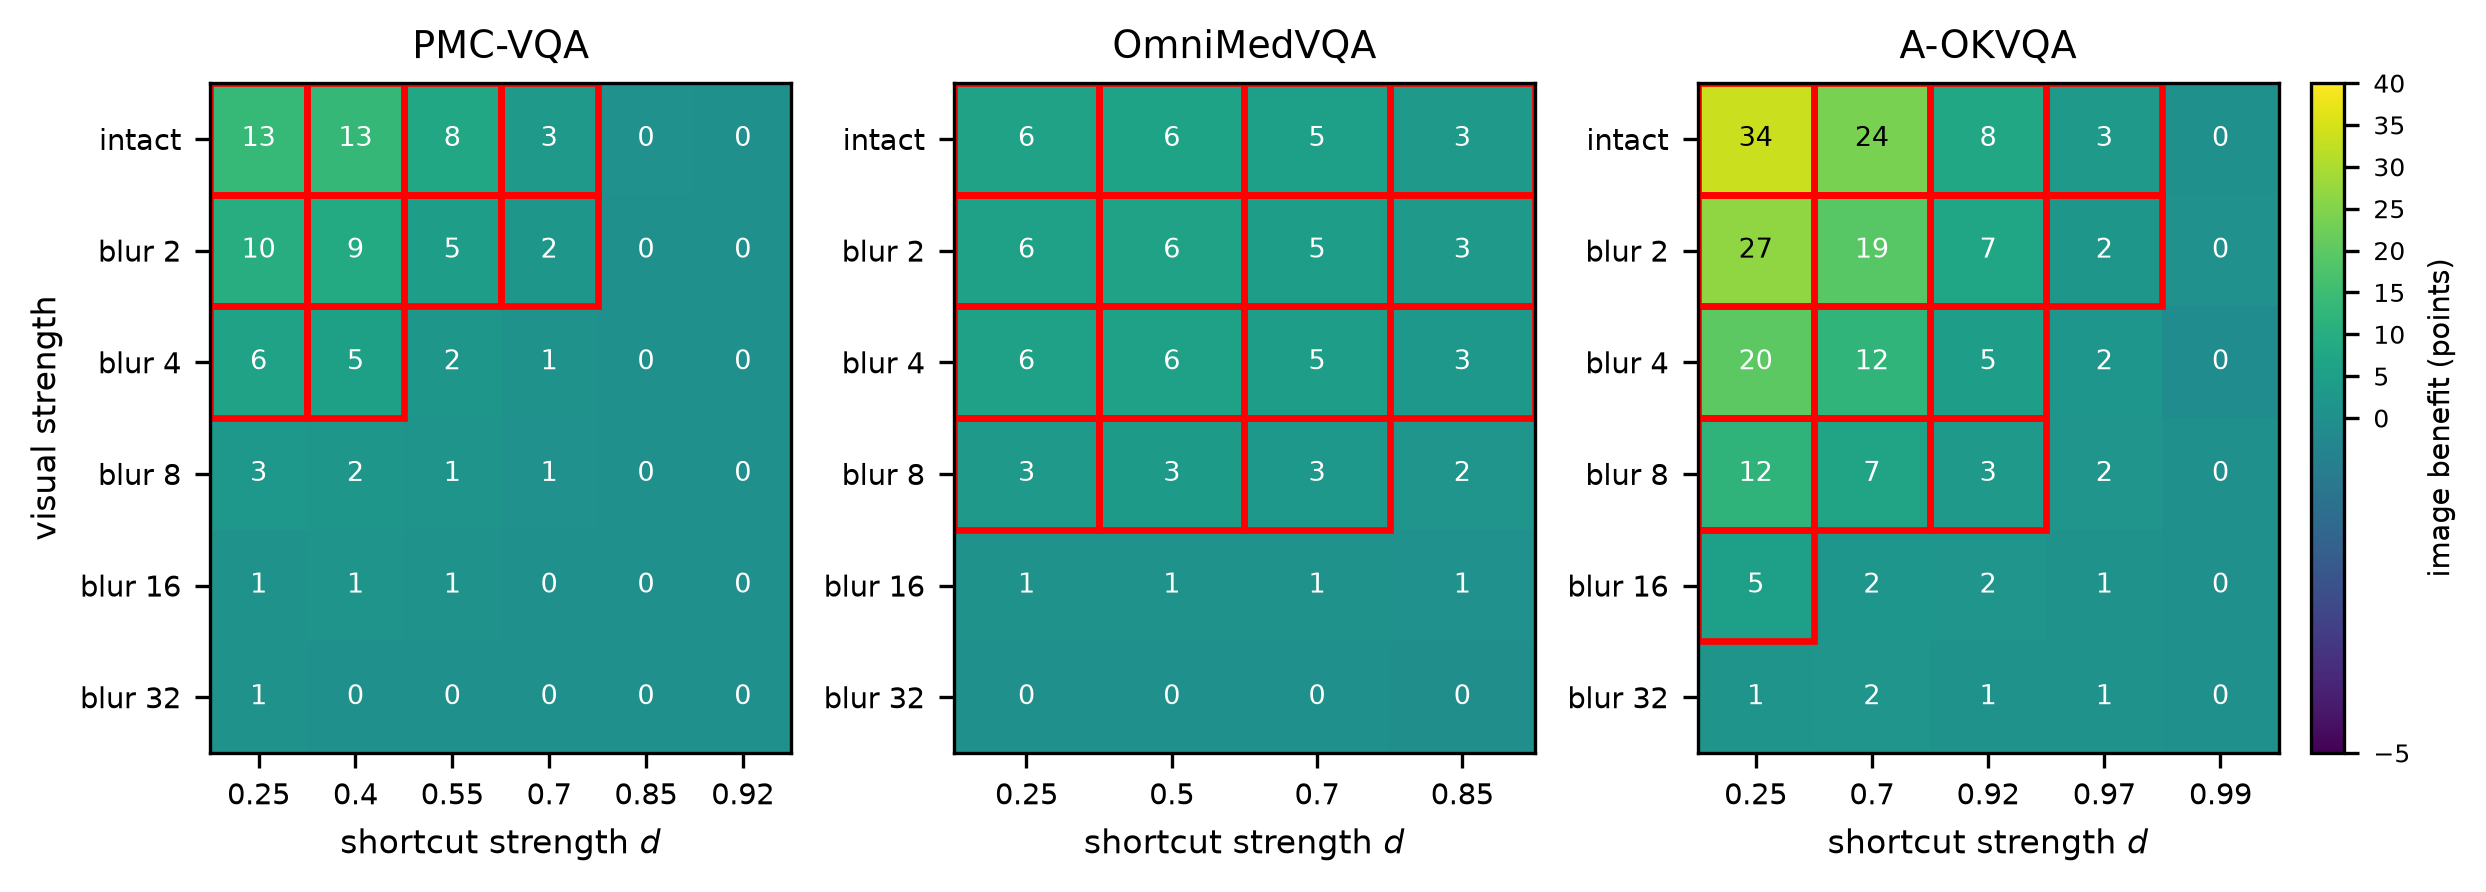
\includegraphics[width=0.78\textwidth]{fig/f12_phase.png}
  \caption{\textbf{Phase diagram of image use} (planted length shortcut, Qwen2.5-VL-3B; mean of 2--3 seeds; test sets of 1{,}999, 2{,}000 and 1{,}145 questions). Cells: image benefit, the accuracy with the image at the visual strength of the row (Gaussian blur radius 32, 16, 8, 4, 2\,px on 448\,px images, or intact) minus the accuracy with a black image, in points; columns: the tested shortcut strengths $d$ of each benchmark. Red outline: the visual-veto criterion holds in every seed, i.e.\ the benefit is at least $+2$ points with a paired-bootstrap 95\% lower bound of at least $+1$. A column without outline is a lock-out; it is bracketed by the tested strengths, not fitted: PMC-VQA is locked from $d=0.85$ (unlocked at $0.70$), A-OKVQA at $0.99$ (unlocked at $0.97$), OmniMedVQA is not locked up to $0.85$ (the highest tested).}
  \label{fig:phase}
\end{figure*}

\begin{figure*}[t]
  \centering
  \includegraphics[width=\textwidth]{fig/f10_domains.pdf}
  \caption{\textbf{Shortcut strength and visual control in two domains} (planted length shortcut). (a)~Image benefit of the intact image against the shortcut strength $d$ (logit scale), PMC-VQA (blue; Qwen-3B three seeds, InternVL3-2B and Qwen-7B two seeds) and A-OKVQA (green; Qwen-3B three seeds, Qwen-7B and InternVL3-2B two seeds). (b)~Veto boundary $V^\ast$ (mean over seeds; \emph{none}: no tested image strength helps). (c,d)~Benefit along the visual ladder (Qwen-3B): where the shortcut is strong the image helps only when it is intact or nearly so, or not at all.}
  \label{fig:dose}
\end{figure*}

\paragraph{The image benefit falls with the dose.}
On PMC-VQA the benefit of the intact image falls monotonically from $+13.5$ points at $d=0.25$ to $+13.2$, $+8.0$, $+3.4$, $+0.4$ and $+0.1$ points at $d=0.92$ (Fig.~\ref{fig:dose}a; pooled Spearman $\rho=-0.96$, permutation $p<10^{-4}$, Holm-corrected; every seed $\rho\le-0.94$).
At the same time the model learns the shortcut (picks the shortest option 22\%, 42\%, 75\%, 92\%, 99\%, 99\% of the time), its text-side margin rises from $0.25$ to $3.25$ log-odds, and its accuracy on the original, cue-free options falls from 52\% to 38\% (Supp.~Q).
The veto boundary shifts with it (Fig.~\ref{fig:dose}b,c): at $d=0.25$ a blur of radius 8 or 4 already gives a benefit; at $d=0.55$--$0.70$ only a blur of radius 4 or 2 does; for $d\ge0.85$ no image strength qualifies (none in all three seeds; $\rho(d,V^\ast)=+0.94$, Holm-corrected).

\paragraph{The same intervention on natural photographs.}
On A-OKVQA the correct option is the shortest in only 16.1\% of the test questions.
Between $d=0.25$ and $0.92$ the benefit falls from about $+34$ to $+8$ points (Qwen-3B $+33.9\to+8.1$, Qwen-7B $+34.2\to+6.5$, InternVL3-2B $+37.6\to+11.7$).
At $d=0.97$ and $0.99$, tested after seeing this with criteria fixed beforehand, the benefit of Qwen-3B is $+2.5$ to $+3.3$ and $+0.1$ to $+0.35$ points with no helpful image strength in three seeds, and Qwen-7B behaves alike; InternVL3-2B keeps $+1.7$ points at $0.99$.
The lock-out strength is thus not a constant ($0.85$ for Qwen-3B on PMC-VQA, $0.99$ for the Qwen models on A-OKVQA) and is not ordered by the benefit without a cue (Sec.~\ref{sec:general}; Supp.~Y).
A position shortcut and a centre-versus-border occlusion are in Supp.~Q and Z; attempts to explain the boundary are in Sec.~\ref{sec:general}.
